\subsection{Metabolisme bag fysisk aktivitet}
%{\color{red}\textbf{Vi vil forsøge at gøre dette afsnit mere problemorienteret. Hvis ikke dette kan lade sig gøre, vil afsnittet komme ind som bilag.}}
Ved fysisk aktivitet kræver musklerne energi. Dette sker ved fraspaltning af en fosfatgruppe (P) fra adenosintrifosfat (ATP), som derefter bliver til adenosindifosfat (ADP). ATP skal derfor gendannes konstant, hvilket kan foregå under aerobe eller anaerobe forhold.\fxnote{Anaerob=uden ilt, aerob=med ilt} Under anaerobe forhold er der ikke tilstrækkelig ilt til stede, hvorfor denne proces er den første, som indtræder under fysisk aktivitet. ATP kan gendannes anaerobt ved spaltning af kreationfosfat eller kulhydrater under dannelse af mælkesyre. Disse processer kaldes overordnet for glykolysen og finder sted i cytosolen i muskelcellerne ved fysisk aktivitet. Der dannes ATP samt en række andre stoffer, som skal indgå i citronsyrecyklusen og den oxidative fosforylering.\citep{Martini2012,Engelbreth2010} \\
Under aerobe forhold kan ATP gendannes i meget store mængder igennem den oxidative fosforylering, hvorfor denne proces for alvor først dominerer efter cirka 15-20 minutter, som kan ses på \figref{fig:Metabolisme}. Den areobe proces foregår i mitokondrierne og kan danne 12 gange mere ATP per gram kulhydrat i forhold til den anaerobe proces, men dette kan dog variere. Effektiviteten af den aerobe proces afhænger, hvor veltrænet kroppen er samt hvor gode musklerne er til at optage den tilførte ilt.\citep{Engelbreth2010,Martini2012,Stanfield2013} 
\begin{figure}[H]
	\centering
	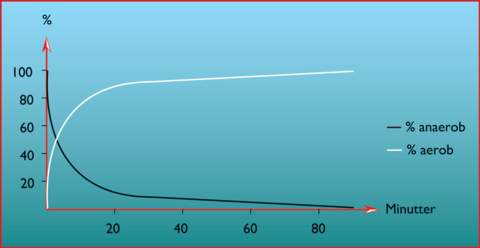
\includegraphics[scale=0.65]{figures/aProblemanalyse/Metabolisme.png}
	\caption{På figuren ses den procentvise fordeling af gendannelsesprocesserne af ATP. Der ses, at efter cirka 20 minutter overtager den aerobe proces.\citep{Engelbreth2010}}
	\label{fig:Metabolisme}
\end{figure}
Glykogen forbrændes først igennem den anaerobe proces i muskelcellerne, hvorfor forbrændingen af dette molekyle er dominerende under intenst arbejde. Fedtforbrænding finder i højere grad sted ved arbejde med lavere intensitet, som er beskrevet i \secref{fig:PA_Procentpuls}.\citep{Martini2012,Stanfield2013,Engelbreth2010}

% http://www.ncbi.nlm.nih.gov/pubmed/15648007
% http://www.ncbi.nlm.nih.gov/pubmed/14692598
% http://www.jrnjournal.org/article/S1051-2276(04)00166-9/pdf
% http://link.springer.com/article/10.1007%2FBF02555089#page-1